O jogo de xadrez possui várias peças com movimentos curiosos: uma delas é a
dama, que pode se mover qualquer quantidade de casas na mesma linha, na mesma
coluna, ou em uma das duas diagonais, conforme exemplifica a figura abaixo:

\begin{center}
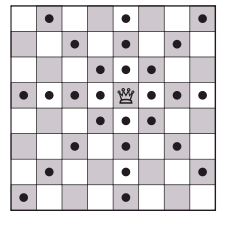
\includegraphics[scale=0.6]{problems/dama/imagens/dama.png}
\end{center}

O grande mestre de xadrez \textit{Kary Gasparov} inventou um novo tipo de problema de
xadrez: dada a posição de uma dama em um tabuleiro de xadrez vazio (ou seja, um
tabuleiro 8 $\times$ 8, com 64 casas), de quantos movimentos, no mínimo, ela
precisa para chegar em outra casa do tabuleiro?

Kary achou a solução para alguns desses problemas, mas teve dificuldade com
outros, e por isso pediu que você escrevesse um programa que resolve esse tipo
de problema.

\subsection*{Entrada}

A entrada contem vários casos de teste. A primeira e única linha de cada caso de
teste contém quatro inteiros X1, Y1, X2 e Y2 (1 $\leq$ X1, Y1, X2, Y2 $\leq$ 8). A
dama começa na casa de coordenadas (X1, Y1), e a casa de destino é a casa de
coordenadas (X2, Y2). No tabuleiro, as colunas são numeradas da esquerda para a
direita de 1 a 8 e as linhas de cima para baixo também de 1 a 8. As coordenadas
de uma casa na linha X e coluna Y são (X, Y).

O final da entrada é indicado por uma linha contendo quatro zeros.

\subsection*{Saída}

Para cada caso de teste da entrada seu programa deve imprimir uma unica linha na
saída, contendo um número inteiro, indicando o menor número de movimentos
necessários para a dama chegar em sua casa de destino.

\begin{table}[!h]
\centering
\begin{tabular}{|l|l|}
\hline
\begin{minipage}[t]{3in}
\textbf{Exemplo de entrada}
\begin{verbatim}
4 4 6 2
3 5 3 5
5 5 4 3
0 0 0 0
\end{verbatim}
\vspace{1mm}
\end{minipage}
&

\begin{minipage}[t]{3in}
\textbf{Exemplo de saída}
\begin{verbatim}
1
0
2
\end{verbatim}
\vspace{1mm}
\end{minipage} \\
\hline
\end{tabular}
\end{table}

\newpage
